\documentclass[11pt]{article}
\usepackage[margin=1in]{geometry}
\usepackage[T1]{fontenc}
\usepackage{lmodern}
\usepackage{microtype}
\usepackage{amsmath}
\usepackage{booktabs}
\usepackage{graphicx}
\usepackage{xcolor}
\usepackage{enumitem}
\usepackage[hidelinks]{hyperref}
\usepackage[numbers,sort]{natbib}
\setlist{nosep,leftmargin=1.4em}

\title{One Judge, Same Probes: Re-evaluating Agentic Memory on ATLAS\\
and a Three-Agent Retrieve--Answer--Verify Loop}
\author{Mycelic Labs}
\date{November 2026}

\begin{document}
\maketitle

\begin{abstract}
ATLAS is a public benchmark for agentic memory systems: 1{,}092 probes over 100 synthetic multi-session worlds, scored by an LLM judge. Its published results rank Nebula first (82.0\% simple, 71.0\% complex). We audit those results and find the arithmetic exact. However, the files do not record the answer model, the judge model, or the code version, and the judge is inconsistent: identical ``Unknown''/``Unknown'' pairs were marked wrong in 31 of 65 cases. We re-score every published answer with a single judge (Claude Opus) that is blind to which system wrote the answer and uses the benchmark's own judge prompts. The ranking is preserved, and all systems gain 2--7 points. We then evaluate a three-agent memory loop: a deterministic hybrid retriever, an Answerer, and a Verifier that can trigger a second retrieval round. With Opus as the answer model it reaches 96.1\% (simple) and 93.8\% (complex). Two controls use the same answer model and the same judge. Against naive RAG the loop gains +19.0 and +21.1 points on held-out files. Against putting the full history in context it gains +7.5 points on simple (95\% CI +1.5 to +14.8) and +4.2 points on complex, which is not significant (CI $-1.6$ to $+11.6$), while using about 31\% of the full-history context on complex. Because the published systems answered with GPT-4o-class models, and full-context Opus alone already exceeds the published Nebula scores, we do \emph{not} claim that our memory system outperforms Nebula's memory system. We release all prompts, retrieval code, per-probe answers, traces and verdicts.
\end{abstract}

\section{Introduction}
Memory benchmarks for LLM agents compare whole systems: an ingestion pipeline, a retriever, an answer model and a judge. When those components differ between entries, a leaderboard gap can come from any of them. ATLAS~\citep{atlas2026} is a recent benchmark of this kind. It organizes probes into six cognitive \emph{pillars} (world modeling, declarative reasoning, temporal/episodic memory, preference learning, knowledge boundaries, procedural knowledge) and publishes per-probe results for Nebula, Supermemory, Mem0 and a naive RAG baseline.

This report makes three contributions:
\begin{enumerate}
\item \textbf{An audit of the published results} (\S\ref{sec:audit}). We recompute every score, check coverage against the test sets, and characterize judge inconsistency.
\item \textbf{A single-judge re-score} (\S\ref{sec:rejudge}). All published answers are scored by one blind judge with the benchmark's own prompts. This separates judge effects from system effects.
\item \textbf{A three-agent memory loop with matched controls} (\S\ref{sec:loop}--\ref{sec:results}). We report it alongside naive RAG and full-context baselines that use the same answer model, so that its contribution can be isolated.
\end{enumerate}
We are explicit about what the evidence does and does not support (\S\ref{sec:limits}).

\section{Benchmark and published results}
ATLAS has a \emph{simple} set (50 worlds, 10 sessions each, 589 probes, ${\approx}$3k tokens of history per world) and a \emph{complex} set (50 worlds, ${\approx}$27 sessions each, 503 probes, ${\approx}$9k tokens per world). Answer types are short answer, boolean, verbatim, generation and abstain. Each memory adapter retrieves context for a question. An answer model then produces a short answer, and an LLM judge returns YES/NO against the gold answer using a deliberately lenient prompt. Table~\ref{tab:published} lists the published scores.

\begin{table}[h]
\centering\small
\begin{tabular}{lcc}
\toprule
System & Simple (589) & Complex (503)\\
\midrule
Nebula & 82.0 & 71.0\\
Supermemory & 75.4 & 61.0\\
naive\_rag & 68.8 & 54.9\\
Mem0 & 55.3 & 47.5\\
\bottomrule
\end{tabular}
\caption{Published ATLAS accuracy (\%), recomputed from the released per-probe files.}
\label{tab:published}
\end{table}

\section{Audit of the published results}\label{sec:audit}
A stdlib-only script (\texttt{audit/audit\_published.py}) recomputed every aggregate from the per-probe records. Findings:
\begin{itemize}
\item \textbf{Arithmetic is exact.} All overall, per-pillar, per-answer-type and per-file summaries match the per-probe scores in all eight files.
\item \textbf{Coverage is complete.} Every run covers all 50 files of its set. Probe IDs, order, questions, answer types and gold answers match the current test sets.
\item \textbf{Provenance is missing.} No file records the answer model, judge model or code version. The repository configures a judge model string (\texttt{gemini-3.0-pro}) that falls back to another provider on error, so the judge actually used cannot be determined from the artifacts. The Nebula complex file contains a field (\texttt{scoring\_latency\_ms}) that no code in the repository writes, and the Nebula runs postdate the others by about nine days.
\item \textbf{The judge is inconsistent.} Across all systems, 65 probes have gold ``Unknown'' and prediction ``Unknown''; 31 of them were scored incorrect.
\item \textbf{The judge is lenient.} Some passes do not contain the gold text. For Nebula this is 106 of 384 content probes on simple and 49 of 275 on complex, versus 17--28\% for the other systems. Most of these passes are genuine paraphrases.
\end{itemize}

\section{Single-judge re-scoring}\label{sec:rejudge}
\paragraph{Protocol.} We pooled every (answer type, gold, prediction) triple from all published files and deduplicated them, leaving 1{,}552 unique triples from 4{,}368 scored probes. We then shuffled them (seed 0) and stripped all system identifiers. Judge prompts are generated by calling the repository's own \texttt{llm\_judge\_binary} with the model call intercepted, so the prompt text is byte-identical to the benchmark's. The judge is Claude Opus, run as Claude Code subagents of 194 items each, with verdicts parsed by the repository's own rule (``YES'' $\Rightarrow$ 1). Later items (our systems, \S\ref{sec:results}) were judged the same way, again blind and deduplicated against earlier verdicts. In total there were 2{,}287 unique verdicts.

\paragraph{Results.} Table~\ref{tab:rejudge} shows the effect of the judge change. Every system gains; changes from 0 to 1 dominate (18--34 per run), and changes from 1 to 0 are rare (0--4 per run). The ranking is unchanged, and the Nebula--Supermemory gap is essentially preserved: +7.8 points on simple (+6.6 originally) and +9.3 on complex (+9.9 originally).

\begin{table}[h]
\centering\small
\begin{tabular}{lcccc}
\toprule
& \multicolumn{2}{c}{Simple} & \multicolumn{2}{c}{Complex}\\
\cmidrule(lr){2-3}\cmidrule(lr){4-5}
System & original & Opus judge & original & Opus judge\\
\midrule
Nebula & 82.0 & 87.3 & 71.0 & 76.9\\
Supermemory & 75.4 & 79.5 & 61.0 & 67.6\\
naive\_rag & 68.8 & 73.2 & 54.9 & 61.4\\
Mem0 & 55.3 & 57.7 & 47.5 & 53.9\\
\bottomrule
\end{tabular}
\caption{Published answers, original judge vs.\ one blind Opus judge (accuracy \%).}
\label{tab:rejudge}
\end{table}

\section{A three-agent retrieve--answer--verify loop}\label{sec:loop}
The loop has three roles:
\begin{enumerate}
\item \textbf{Retriever} (deterministic code). Each conversation turn is indexed together with its preceding turn. Two channels rank these units: BM25~\citep{robertson2009bm25} over lightly filtered tokens, and dense cosine similarity with \texttt{bge-small-en-v1.5}~\citep{xiao2023cpack}. Each channel contributes its top 40 units. Rankings are fused with Reciprocal Rank Fusion~\citep{cormack2009rrf} ($k{=}60$). Unit scores are lifted to sessions (best unit plus $0.25\times$ the next two), and the top 8 sessions are returned in chronological order with their timestamps. This mirrors the recall path of NeuralGraph, an open-source memory engine we develop, but it is a separate Python reimplementation, not the NeuralGraph binary.
\item \textbf{Answerer.} It reads the sessions and returns JSON containing a short answer, the cited session IDs and a supporting quote. Its instructions say the latest statement wins when facts change, ordering questions are decided by timestamps, and the answer is ``Unknown'' when the information is absent.
\item \textbf{Verifier.} It checks the draft for support, recency, entity/attribute match and missing information. It then \emph{accepts} the draft, \emph{revises} it from the shown evidence, or \emph{retrieves}: it issues a new query, the Retriever returns up to 4 additional sessions, and the Answerer and Verifier run once more. There are at most two rounds.
\end{enumerate}
Over 1{,}092 probes the Verifier accepted 878 first-round drafts, revised 2 and requested retrieval for 212. Mean evidence shown in round 1 was 11.3k characters on simple and 12.5k on complex. Full histories average 14.7k and 40.2k characters respectively.

\paragraph{What the adapter can see.} The loop receives only the sessions and the question text. It never sees gold answers, answer types, pillars or supporting items.

\section{Experimental setup}\label{sec:setup}
\paragraph{Answer model.} Claude Opus, run as Claude Code subagents. A subagent processes one batch and executes the Answerer and Verifier roles in sequence for each probe, while retrieval is performed by code (precomputed round-1 evidence, plus a local HTTP retriever for round 2). Prompts are listed in Appendix~\ref{app:prompts}.

\paragraph{Controls with the same answer model and judge.}
\begin{itemize}
\item \textbf{naive\_rag (Opus):} the repository's naive RAG retrieval (one document per turn, all-MiniLM-L6-v2, top 10 turns) with the repository's naive RAG prompt.
\item \textbf{Full context (Opus):} the repository's \texttt{no\_rag} prompt with the world's entire history.
\end{itemize}

\paragraph{Leakage controls.} Packets contain only question text and evidence. Each mycelic and naive\_rag batch holds at most one probe per world, so an agent never accumulates evidence from the same world across probes. Full-context batches hold up to 10 whole worlds. We scanned every answer agent's tool calls for access to test sets, result files or verdicts and found none.

\paragraph{Statistics.} Files are split by sorted name into 10 dev and 40 held-out files per set. No prompt or parameter was tuned on any file, so the split is reported only as a check. Paired differences use a 95\% bootstrap CI with resampling clustered by file (10{,}000 resamples, seed 0) and McNemar's exact test~\citep{mcnemar1947}.

\section{Results}\label{sec:results}
\begin{figure}[t]
\centering
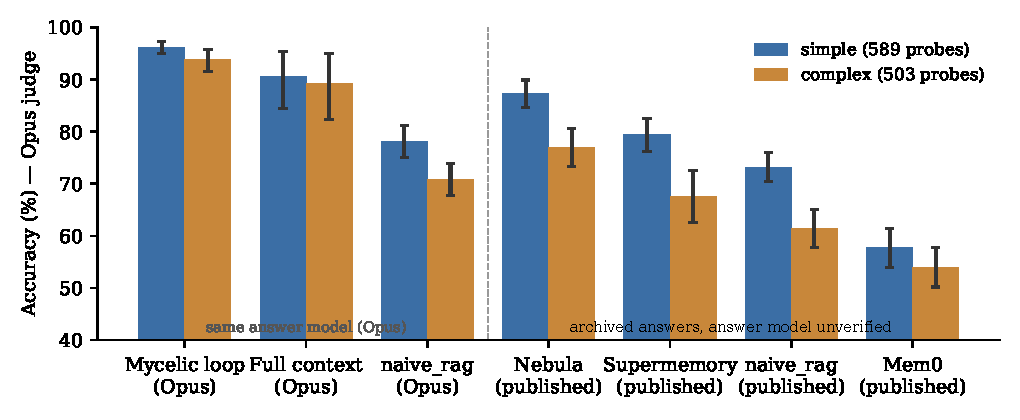
\includegraphics[width=\linewidth]{fig_overall.pdf}
\caption{Accuracy under one blind Opus judge. Error bars: 95\% file-clustered bootstrap CIs. Systems left of the dashed line share the answer model (Opus). Systems to the right are published answers from GPT-4o-class models.}
\label{fig:overall}
\end{figure}

\begin{table}[t]
\centering\small
\begin{tabular}{lll}
\toprule
System & Simple & Complex\\
\midrule
\textbf{Three-agent loop (Opus)} & \textbf{96.1} [94.9, 97.3] & \textbf{93.8} [91.6, 95.7]\\
Full context (Opus) & 90.5 [84.5, 95.3] & 89.3 [82.4, 95.0]\\
naive\_rag (Opus) & 78.1 [75.0, 81.1] & 70.8 [67.7, 73.8]\\
\midrule
Nebula (published answers) & 87.3 [84.6, 89.9] & 76.9 [73.3, 80.6]\\
Supermemory (published answers) & 79.5 [76.2, 82.6] & 67.6 [62.5, 72.5]\\
naive\_rag (published answers) & 73.2 [70.4, 76.0] & 61.4 [57.8, 65.1]\\
Mem0 (published answers) & 57.7 [54.0, 61.4] & 53.9 [50.2, 57.8]\\
\bottomrule
\end{tabular}
\caption{Accuracy (\%) with 95\% file-clustered bootstrap CIs, all probes, one blind Opus judge.}
\label{tab:main}
\end{table}

\begin{table}[t]
\centering\small
\begin{tabular}{llcc}
\toprule
Set & Loop minus & $\Delta$ [95\% CI] & wins / losses ($p$)\\
\midrule
Simple & naive\_rag (Opus) & +19.0 [+15.7, +22.3] & 92 / 3 ($7\times10^{-24}$)\\
 & Full context (Opus) & +7.5 [+1.5, +14.8] & 36 / 1 ($6\times10^{-10}$)\\
 & Nebula (published) & +9.2 [+6.1, +12.4] & 47 / 4 ($2\times10^{-10}$)\\
\midrule
Complex & naive\_rag (Opus) & +21.1 [+17.3, +24.7] & 87 / 6 ($2\times10^{-19}$)\\
 & Full context (Opus) & +4.2 [$-1.6$, +11.6] & 27 / 11 ($0.014$)\\
 & Nebula (published) & +15.9 [+10.6, +20.8] & 74 / 13 ($2\times10^{-11}$)\\
\bottomrule
\end{tabular}
\caption{Paired differences on the 40 held-out files per set (469 simple, 384 complex probes). For the comparison with full context on complex, McNemar's test rejects equality ($p=0.014$) but the file-clustered CI includes zero. We treat that comparison as not significant, because probes within a world are correlated.}
\label{tab:paired}
\end{table}

Table~\ref{tab:main} and Figure~\ref{fig:overall} give overall accuracy, and Table~\ref{tab:paired} gives paired differences on held-out files. Dev and held-out accuracies are close for the loop: 95.0 vs.\ 96.4 on simple and 96.6 vs.\ 93.0 on complex.

\paragraph{Effect of the loop at a fixed answer model.} With Opus fixed, the loop improves on naive RAG by about 20 points on both sets. It also improves on full context on simple. On complex the difference from full context is not significant, but the loop shows the evidence model about 31\% of the characters. Figure~\ref{fig:pillars} shows the largest complex-set gains over naive RAG on temporal/episodic questions (86.7 vs.\ 39.8), preference learning (97.3 vs.\ 62.7) and procedural knowledge (94.7 vs.\ 64.0).

\paragraph{Comparison with published systems.} The loop exceeds Nebula's published answers by 9.2 points on simple and 15.9 on complex (held-out). This comparison is \emph{confounded by the answer model}. Full-context Opus, with no memory system at all, already scores 90.5/89.3, above Nebula's 87.3/76.9. Naive RAG with Opus (78.1/70.8) scores below Nebula, which indicates that Nebula's retrieval is substantially stronger than naive RAG.

\paragraph{Weakness.} On complex-set knowledge-boundary probes, the loop (87.8\%) scores below both Nebula (93.3\%) and full context (90.0\%). We have not yet analysed the cause. One hypothesis is that showing whole sessions makes it easier to answer from loosely related context when the correct answer is ``Unknown''.

\begin{figure}[t]
\centering
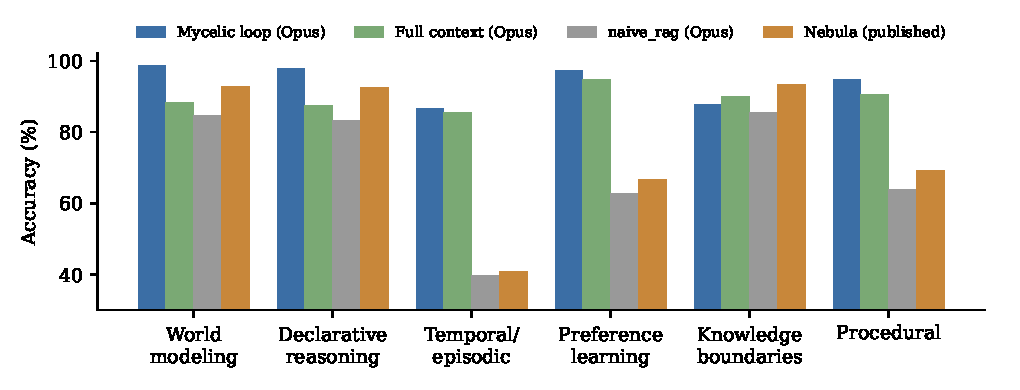
\includegraphics[width=\linewidth]{fig_pillars_complex.pdf}
\caption{Complex set, accuracy by ATLAS pillar under the Opus judge.}
\label{fig:pillars}
\end{figure}

\paragraph{Judge-free cross-check.} Because the judge and the answer model are the same model family, we also report a metric without any judge: whether the normalized gold text appears in the prediction (short-answer and verbatim probes). The ordering holds. The loop scores 71.5\% (simple) and 74.6\% (complex), full context 68.4/71.7, Nebula 60.7/56.3, and naive RAG (Opus) 52.9/54.9. Mean answer length is 19.2/17.8 characters for the loop and 19.8/18.5 for full context, and no prediction from the loop hedges between multiple options.

\section{Limitations}\label{sec:limits}
\begin{itemize}
\item \textbf{Answer model.} The comparison with published systems mixes memory systems and answer models. A like-for-like comparison would run Nebula with Opus, or the loop with the published answer model. We could do neither, because we had no access to the Nebula service or to the published models' API.
\item \textbf{Same model family.} Opus judges answers that Opus wrote. Judging was blind and the judge-free metric agrees, but self-preference effects~\citep{zheng2023judge} cannot be excluded entirely.
\item \textbf{Execution through subagents.} The Answerer and Verifier ran as roles within one subagent context per batch, not as separate API calls. A full-context batch holds up to ${\sim}$110 questions over 10 worlds, which may disadvantage that control relative to per-question calls. One answer agent reported briefly seeing two scratch files of another agent from unrelated worlds. It reported not using them, and the one-probe-per-world batching limits the possible effect.
\item \textbf{Reproducibility.} Retrieval, packets, prompts and the judge prompt are deterministic and released. LLM outputs are not bit-reproducible; we release every answer, trace and verdict so results can be re-scored, and the judge can be re-run against the API with \texttt{scripts/opus\_judge.py api}.
\item \textbf{Prototype.} The loop is a research prototype. It is not a shipped Mycelic or NeuralGraph product feature.
\item \textbf{Benchmark difficulty.} ATLAS histories fit comfortably in a frontier model's context window, so its ceiling tests a memory system less than a long-horizon benchmark would~\citep{maharana2024locomo,wu2024longmemeval}.
\end{itemize}

\section{Conclusion}
A single blind judge preserves the published ATLAS ranking and removes judge noise. With the answer model held fixed, a simple three-agent retrieve--answer--verify loop beats naive RAG by about 20 points, and matches or beats full context while reading a third as much on the larger worlds. The headline gap over published systems is real on these probes, but it is not evidence that one memory system beats another. Settling that requires running every system with the same answer model.

\paragraph{Artifacts.} \url{https://github.com/anovruzov/atlas-bench}: \texttt{audit/}, \texttt{judge/}, \texttt{opus\_run/} (answers, traces, results), and \texttt{scripts/} (\texttt{opus\_packets.py}, \texttt{opus\_judge.py}, \texttt{opus\_compare.py}, \texttt{atlas\_repro.py}).

\bibliographystyle{plainnat}
\begin{thebibliography}{9}
\bibitem[Nebula(2026)]{atlas2026} Nebula. \newblock {ATLAS}: Cognitive-based benchmarking for agentic memory systems. \newblock Software and data, 2026.
\bibitem[Robertson and Zaragoza(2009)]{robertson2009bm25} S.~Robertson and H.~Zaragoza. \newblock The probabilistic relevance framework: {BM25} and beyond. \newblock \emph{Foundations and Trends in Information Retrieval}, 3(4):333--389, 2009.
\bibitem[Cormack et~al.(2009)]{cormack2009rrf} G.~V. Cormack, C.~L.~A. Clarke, and S.~B{\"u}ttcher. \newblock Reciprocal rank fusion outperforms {Condorcet} and individual rank learning methods. \newblock In \emph{SIGIR}, 2009.
\bibitem[Xiao et~al.(2023)]{xiao2023cpack} S.~Xiao, Z.~Liu, P.~Zhang, and N.~Muennighoff. \newblock {C-Pack}: Packaged resources to advance general {Chinese} embedding. \newblock arXiv:2309.07597, 2023.
\bibitem[McNemar(1947)]{mcnemar1947} Q.~McNemar. \newblock Note on the sampling error of the difference between correlated proportions or percentages. \newblock \emph{Psychometrika}, 12(2):153--157, 1947.
\bibitem[Zheng et~al.(2023)]{zheng2023judge} L.~Zheng et~al. \newblock Judging {LLM-as-a-judge} with {MT-Bench} and {Chatbot Arena}. \newblock In \emph{NeurIPS Datasets and Benchmarks}, 2023.
\bibitem[Maharana et~al.(2024)]{maharana2024locomo} A.~Maharana, D.-H. Lee, S.~Tulyakov, M.~Bansal, F.~Barbieri, and Y.~Fang. \newblock Evaluating very long-term conversational memory of {LLM} agents. \newblock In \emph{ACL}, 2024.
\bibitem[Wu et~al.(2024)]{wu2024longmemeval} D.~Wu, H.~Wang, W.~Yu, Y.~Zhang, K.-W. Chang, and D.~Yu. \newblock {LongMemEval}: Benchmarking chat assistants on long-term interactive memory. \newblock arXiv:2410.10813, 2024.
\end{thebibliography}

\appendix
\section{Prompts}\label{app:prompts}
\paragraph{Answerer.}\begin{small}\begin{verbatim}
You are the Answerer in a memory system. You receive excerpts of past
conversations between a user and an assistant, shown in chronological
order (higher t = later). Answer the question using ONLY these
conversations. Rules:
- If facts changed over time, the latest statement wins unless the
  question asks about an earlier time.
- For "before/after" or ordering questions, compare the t values.
- If the conversations do not contain the information, the answer is
  "Unknown". Do not guess.
- The answer must be as short as possible. No explanation.
Reply with JSON only: {"answer", "sessions", "quote"}
\end{verbatim}\end{small}
\paragraph{Verifier.}\begin{small}\begin{verbatim}
You are the Verifier in a memory system. Check the draft strictly:
1. directly supported (not just plausible)?  2. latest value?
3. right entity and attribute?  4. if absent, the answer is "Unknown".
Reply with JSON only: {"verdict": accept|revise|retrieve,
"final_answer", "search_query", "reason"}
\end{verbatim}\end{small}
The full prompt text is in \texttt{benchmark/evaluation/mycelic\_loop.py}. The judge prompts are those of \texttt{benchmark/evaluation/metrics.py}, unchanged.
\end{document}
